\section{Inleiding}
Het programma is een toepassing van \textit{Decision tree learning}.\cite{wiki:dtl} Dit houd in dat we via machine-learning een zogenoemde \textit{decision tree} op bouwen. Dat is een boomstructuur die beslissing maakt op basis van observaties om zo tot een conclusie te komen.

\begin{figure}[ht]
    \centering
    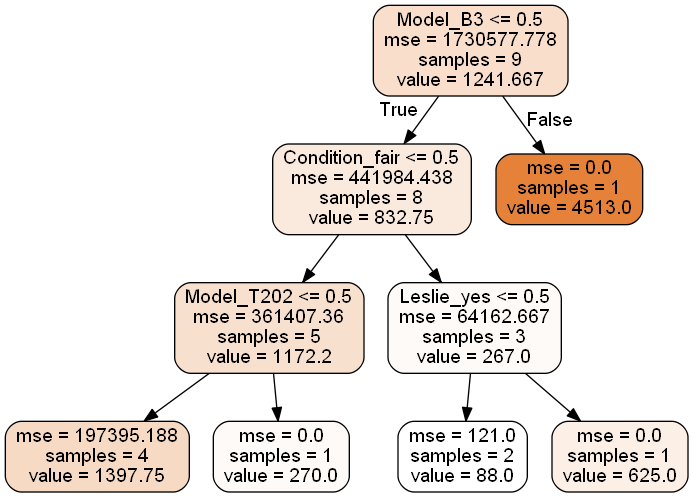
\includegraphics[width=0.8\textwidth]{illustraties/tree}
    \caption{Een voorbeeld van zo'n \textit{decision tree}.}
    \cite{git:github}
    \label{fig:tree}
\end{figure}

De boom in Figuur \ref{fig:tree} is opgesteld door een Python script. Hij berekend de prijs van orgels. Python is een geweldige taal om snel machine-learningapplicaties te prototypen.Toch mist Python de performantie die nodig is om hoge aantalen orgels te prijzen. Daarvoor gaan we de boom coderen naar een JSON-formaat. Dat kunnen we dan decoderen in een C++ programma. C++ heeft namelijk de performantie die we nodig hebben. Tegenover Python is C++ wel een stuk complexer.

\clearpage

\section{Boomstructuur}
De boomstructuur start met één Tree-object (Blauw in Figuur \ref{fig:cpp-tree}). Deze heeft een pointer, genaamd ``root'' naar een TreeNode-object. Elke TreeNode heeft twee pointers naar andere TreeNodes. Namelijk ``trueNode'' en ``falseNode''. Als deze pointers daadwerkelijk verwijzen naar andere TreeNodes hebben we een brach-node (Rood in Figuur \ref{fig:cpp-tree}). Bij sommige TreeNodes wijzen de pointer nergens heen. Dan hebben we een zogenoemde leaf-node (Groen in Figuur \ref{fig:cpp-tree}).

\begin{figure}[ht]
    \centering
    \small
    \begin{tikzpicture}[
        tree/.style={circle, draw=blue!60, fill=green!5, very thick, minimum size=7mm},
        branch/.style={rectangle, draw=red!60, fill=red!5, very thick, minimum size=5mm},
        leaf/.style={rectangle, draw=green!60, fill=red!5, very thick, minimum size=5mm},
        ]
        %Nodes
        \node[tree]     (main)                                  {Tree};
        \node[branch]   (root)          [below=of main]         {root : TreeNode};
        \node[branch]     (trueNode)   [below left=1.5cm and 0.1cm of root]   {trueNode : TreeNode};
        \node[leaf]   (falseNode)   [below right= 1.5cm and 0.1cm of root]    {falseNode : TreeNode};
        
        \node[leaf]   (falseNode2)   [below right= 1.5cm and 0.1cm of trueNode]    {falseNode : TreeNode};
        \node[leaf]     (trueNode2)   [below left=1.5cm and 0.1cm of trueNode]   {trueNode : TreeNode};
        
        %Lines
        \draw[<-] (root.north) -- (main.south);
        \draw[<-] (trueNode.north) -- (root.south);
        \draw[<-] (falseNode.north) -- (root.south);
        \draw[<-] (trueNode2.north) -- (trueNode.south);
        \draw[<-] (falseNode2.north) -- (trueNode.south);
        \end{tikzpicture}

    \caption{De boomstructuur zoals in het C++-programma.}
    \label{fig:cpp-tree}
\end{figure}

\pagebreak
\section{JSON}
De regressieboom wordt gegenereerd in python. Deze wordt dan gecodeerd en weggeschreven in JSON-formaat. Voor het inlezen van data in JSON-formaat bestaan al goede bibliotheken. Toch hebben we gekozen om dit zelf te programmeren. Wij waren namelijk ook intrinsiek gemotiveerd uit te zoeken hoe zo'n parser zou kunnen werken.

\begin{figure}[ht]
    \centering
    \lstinputlisting[language=JavaScript]{code/rules_d2.json}
    \caption{De boomstructuur in JSON-formaat.}
    \label{fig:json_tree}
\end{figure}

Zoals te zien op Figuur \ref{fig:json_tree}, heeft elke node twee zogenoemde \textit{key-value pairs} of sleutel-waardeparen: \lstinline[language=JavaScript]{"key": "value"}. 
Deze zijn telkens gescheiden door komma's. Deze paren staan in een onbepaalde volgorde. Tijdens het lezen moeten we dus controleren waar elke sleutel voor staat.

\subsection{Sleutel: ``name''}
In deze sleutel staat een string met daarin de prijs of de beslissingsvoorwaarden gecodeerd. Hoe we deze decoderen staat uitgelegd in sectie \ref{sec:regex}.
\subsection{Sleutel: ``children''}
Als er \lstinline[language=JavaScript]{null} in deze sleutel staat, betekend het dat de node geen childnodes heeft. Dan moet staat er ook een prijs gecodeerd in de sleutel \lstinline[language=JavaScript]{"name"}.
Het kan ook dat er een lijst met twee childnodes in staat. Dan hebben we een beslissingsnode waarbij de beslissingsvoorwaarden in de sleutel \lstinline[language=JavaScript]{"name"} staat.

\section{Inladen van de structuur}
Met de functie ``\lstinline[language=C++]{void Tree<T>::load(const string& filename)}'' maakt het Tree-object een ifstream, of input file stream, van de gegeven file. Dan wist hij de vorige boom uit het geheugen. Zo kan dit Tree-object een nieuwe boom aanmaken zonder memory-leaks. Om deze boom in te lezen, haalt hij simpelweg de juiste constructor van de TreeNode aan. \\
Namelijk  ``\lstinline[language=C++]{TreeNode<T>::TreeNode(std::ifstream& fileStream)}''. Daarna steekt hij deze TreeNode in de ``root''-pointer.

In deze constructor gaat het TreeNode-object de ifstream uitlezen. Dat doet hij karakter per karakter. Als hij een sleutel tegenkomt, kijkt hij welke het is. Daarna leest hij op een correcte manier de waarde die bij deze sleutel hoort. De waarde bij de sleutel \lstinline[language=JavaScript]{"name"} wordt simpelweg uitgelezen als string en opgeslagen om later de data uit te halen met regex (zie sectie \ref{sec:regex}). De lijst met child-nodes bij de sleutel \lstinline[language=JavaScript]{"children"} lezen we per node recursief uit.

We halen namelijk ook recursief dezelfde constructor aan:
\nopagebreak

``\lstinline[language=C++]{TreeNode<T>::TreeNode(std::ifstream& fileStream)}''
\nopagebreak

Dat doen we met dezelfde ifstream. Zo vertrekt de child-node met lezen waar wij gestopt waren. Als de child-node dan klaar is, staat de ifstream automatisch bij de volgende node in de lijst.
Deze recursie stop bij elke leaf-node, waarbij er \lstinline[language=JavaScript]{null} in de sleutel \lstinline[language=JavaScript]{"children"} staat.


\section{Regex} \label{sec:regex}
De beslissingsvoorwaarden of de prijs wordt opgeslagen in een string. Om deze data snel en foutloos uit deze string te halen gebruiken we regular expressions oftewel regex. Een zogenoemde regular expression is een reeks karakters die samen een patroon definiëren. Zo'n patroon wordt gebruikt om bepaalde dingen te zoeken, om speciefieke dingen te veranderen of om inputs te controleren.\cite{wiki:regex}

\subsection{Prijs}
\begin{figure}[ht]
    \centering
    \begin{lstlisting}[language=JavaScript]
{
    "name": "267 of Price",
    "children": null
}
        \end{lstlisting}
    \caption{De JSON van een prijsnode.}
    \label{fig:json_leaf}
\end{figure}


Om hier de prijs uit de naam van de node in Figuur \ref{fig:json_leaf} te halen hebben we deze regular expression geschreven: \lstinline{"(.*) of Price"}. Dit komt overeen met elke string die eindigt op `` of Price''. Alles wat er voor komt vangen we op in de capture group. Zo'n capture group is een paar haakjes en alles wat er in staat: \lstinline{"(.*)"}.\cite{Goyvaerts2017} Het getal in die capture group kunnen we dan uitlezen en opslaan.

\subsection{Beslissing}
\begin{figure}[ht]
    \centering
        \begin{lstlisting}[language=JavaScript]
{
    "name": "Model_B3 > 0.5",
    "children": [{...}, {...}]
}
        \end{lstlisting}
    \caption{De JSON van een beslissingsnode.}
    \label{fig:json_branch}
\end{figure}

Het extraheren van de beslissingsvoorwaarden is een stuk complexer. Hiervoor gebruiken we deze regular expression: 

\lstinline{"(.*)_(.*) ([><]) ([-+]?[0-9]*\.?[0-9]*)"}

De eerste en tweede capture group bepaald resp. het attribuut en welke waarde het moet hebben. De derde bepaald de vergelijkingsoperator. De laatste capture group vangt een kommagetal op.

\section{Testen}
In dit deel wordt getest hoe goed de pijsbepaling gebeurt bij bepaalde boomdieptes. Er wordt ook getest wat de invloed is van de boomdiepte op de tijd die het programma nodig heeft om de boom in te laden en om de prijs te bepalen. 

Om een zo accuraat mogelijk resultaat te bekomen, hebben we elke boom tienduizend, \(10^4\), keer ingeladen. Ook voor elke boom hebben we tien miljoen, \(10^7\), orgels geprijsd. De test duurde in totaal \(8.15613\) seconden. De resultaten zijn te zien in Tabel \ref{fig:test_result}.

\begin{table}[ht]
    \small
    \centering
    \begin{tabular}{|c|r|r|r|r|l|}
        \hline
        \bfseries Depth & \bfseries Load time & \bfseries Estimate time & \bfseries Total error & \bfseries Abs. error & \bfseries Rel. error\\
        \hline
        \csvreader[head to column names, late after line=\\]{data.csv}{}%
        {\depth & \load s & \est s & \total & \abs & \rel \%}
        \hline
    \end{tabular}
    \caption{Testresultaten.}
    \label{tab:test_results}
\end{table}

De inlaadtijd van de boom is duidelijk afhankelijk van de boomdiepte. Bij een diepere boom zien we een duidelijke stijging in inlaadtijd. Met de grote-O-notatie is dit een complexiteit van $ O({2^n}) $. In dit geval is het geen worst case scenario omdat de boom niet overal vertakt tot beneden.

Bij het bepalen van de prijs zien we ook dat het langer duurt bij een diepere boom.

Bij het testen gebruiken we alleen orgels waarvan we de prijs kennen. Het programma maakt dan de schatting van de prijs. Deze prijs wordt dan vergeleken met echte prijs. Bij het nemen van de absolutewaarde van de fout en hier het gemmiddelde van te nemen over alle orgels krijgen we de absolute fout die te vinden is in de tabel. Het is heel dijdelijk dat deze fout kleiner wordt als de boom dieper wordt. Dit komt natuurlijk door dat er meer beslissing worden genomen en dus een betere prijsschating kan worden gedaan. Als we dan naar de procentuele fout gaan kijken, is deze bij een diepte van 5 heel klein. Daaruit kunnen we besluiten dat we bij een diepte van 5 een precise bepaling hebben van de pijs.

\begin{figure}[ht]
    \centering
    \begin{tikzpicture}
        \begin{axis}[
            width=0.7\textwidth,
            xlabel={Boom diepte },
            ylabel={Gem. ladingstijd (s)}]
            \addplot table [col sep=comma, x=depth , y=load] {data.csv};
        \end{axis}
    \end{tikzpicture}

    \begin{tikzpicture}
        \begin{axis}[
            width=0.7\textwidth,
            xlabel={Boom diepte },
            ylabel={Gem. uitvoertijd (s)}]
            \addplot table [ col sep=comma, x=depth, y=est] {data.csv};
        \end{axis}
    \end{tikzpicture}

    \caption{Grafieken van de testresultaten.}
    \label{fig:test_result}
\end{figure}

\subsection{Testomgeving}
In Tabel \ref{tab:pc-specs} staan de specificaties van de gebruikte computer. Van alle computers waarop we de test konden uitvoeren, was deze computer de snelste.

\begin{table}[ht]
    \centering
    \begin{tabular}{|l|l|}
        \hline
        \multicolumn{2}{|l|}{\bfseries Software} \\
        \hline
        VS Build configuration  & Release x64 \\
        Besturingssysteem       & Windows 10 Pro 64-bit (10.0, Build 17763) \\
        \hline
        \hline
        \multicolumn{2}{|l|}{\bfseries Hardware} \\
        \hline
        Processor               & Intel Core i7-7700K CPU @ 4.60 GHz OC (8 CPU's) \\
        Geheugen (RAM)          & 2x8.0 GB @ 2933 MHz \\
        Grafische kaart         & NVIDIA GeForce GTX 1080 Ti \\
        \hline
    \end{tabular}
    \caption{Specificaties van de gebruikte computer.}
    \label{tab:pc-specs}
\end{table}

\clearpage

\section{Teamwerk}
Één programma schrijven met meerdere programmeurs is niet simpel. Daarom gebruiken wij twee belangrijke tools. Met deze tools konden wij ons meer focussen op het programma zelf en minder op het oplossen van randproblemen.

\subsection{Git}
De eerste tool die wij gebruiken is Git.
Git is een \textit{Version Control System} (VCS) oftewel een versiebeheersysteem. De oorspronkelijke ontwikkelaar van git is Linus Torvalds in 2005.\cite{git:init} Ondertussen werken er al veel meer ontwikkelaars aan.

In een zogenoemde \textit{Git repository} worden alle verandering van code onthouden. Deze veranderingen slaagt men als programmeur op per nieuwe revisie. Deze revisies worden allemaal bijgehouden op chronologische volgorde. Zo kan men teruggaan naar een vorige revisie en deze vergelijken met de nieuwere revisie. Zo kan men de oorzaak van een fout sneller opsporen.

\subsection{Github}

De website \textit{www.github.com}, oftewel Github, is de tweede tool.
Deze website is een online platform voor versiebeheer via Git. Via Github kunnen programmeurs hun \textit{repository} online opslaan.\cite{git:hello_world} Zo kunnen zij altijd en overal aan hun code en deze ook snel delen met andere programmeurs.

\begin{figure}[ht]
    \centering
    
\includegraphics[width=0.4\textwidth]{illustraties/Octocat}
    \caption{Octocat, de mascotte van GitHub.}
    \cite{git:github}
    \label{fig:octocat}
\end{figure}

% We fixen de positie van deze figuur nog wel
